\chapter{热力学第二定律}
\thispagestyle{empty}
热力学过程中过程的方向性和能量的可逆性是第一定律无法解决的,热力学第二定律可以很好的解释这个现象。
\section{过程不可逆性的现象}
\noindent 大量事实表面:自然过程具有方向性。例如:
\begin{itemize}
	\item 高温的物体能\textbf{自动}地向低温物体传递热量,而低温物体则不能自动向高温物体传递热量。
	\item 水自动地向低处流,而不能自动向高出柳。
	\item 在密闭容器中两种不同的气体可以自动地混合成均匀的混合气体,而不能自动地分离成两个单一的气体。
\end{itemize}

\defination[不可逆过程]
当系统完成某一过程时所产生的效果没不能在其逆过程中得以完全消除,会留下某些影响,则该过程为\dy[不可逆过程]{BKNGC}。

\warn[
\hspace*{2em}不可逆过程不是不可逆行的过程。
]

产生不可逆过程的因素称为\dy[不可逆因素]{BKNYS}。
\begin{equation*}
	\mbox{不可逆因素}\,\,
	\begin{cases}
		\,\,\mbox{\dy[有限势差]{YXSC}}\\
		\,\,\mbox{\dy[耗散效应]{HSXY}}
	\end{cases}
\end{equation*}

\defination[可逆过程]
当系统完成某一过程时所产生的效果,能在其逆过程中得以完全消除,而不留下任何影响,则该过程为\dy[可逆过程]{KNGC}。

可逆过程是自然过程中不可逆过程趋于无限小的极限情况。

可逆过程是一种理想化过程,而严格来说,自然界的一切过程都是不可逆过程,但这一理想化过程为热力学研究提供了方便。

下面介绍两个例子:气体的自由膨胀和有摩擦的热力学过程。

\newpage
\subsection{自由膨胀}
\noindent 在如图\ref{自由膨胀}的装置中,
\begin{itemize}
	\item 若A中存在气体,B为真空
	\begin{itemize}
		\item 由于A和B之间存在一个有限压差,释放隔板后,气体会自由膨胀,将隔板推导右端,由于$p_b = 0$,所以膨胀功$W = 0$
		\item 若将隔板左移至原来的位置,使系统恢复原态,是不可能自动进行的,必须外加压缩功。
		\item 这是不可逆过程。
	\end{itemize}
	\item 若A和B中的气体压力相近
	\begin{itemize}
		\item A气体在膨胀过程中,始终保持与系统B的压力相近,其为准平衡状态,则膨胀功为$\displaystyle W = \int p \, \d v$
		\item 若在B系统中添加与系统A相近的压力使隔板左移至原来的位置,使系统恢复原态,也为准平衡状态,则膨胀功为$\displaystyle W = -\int p \, \d v$
		\item 这是可逆过程。
	\end{itemize}
\end{itemize}
所以,有限的压力差是造成过程不可逆的因素,且压力差越大,不可逆程度也越大。
\vspace*{0.5em}
\begin{figure}[!htb]
	\begin{minipage}{0.5\linewidth}
		\centering
		
\includegraphics[width=0.5\linewidth]{pic/自由膨胀.pdf}
		\caption{自由膨胀装置图}
		\label{自由膨胀}
	\end{minipage}
	\begin{minipage}{0.5\linewidth}
		\centering
		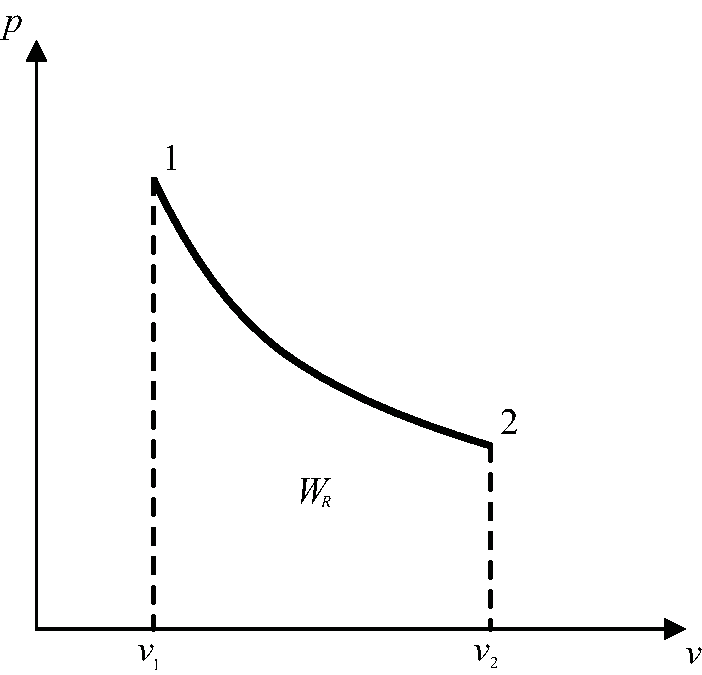
\includegraphics[width=0.62\linewidth]{pic/摩擦.pdf}
		\caption{活塞闭系曲线图}
		\label{活塞闭系曲线}
	\end{minipage}
\end{figure}
\subsection{有摩擦的过程}
\noindent 对于活塞气缸围成的闭系,如图\ref{活塞闭系曲线}.
\begin{itemize}
	\item 无摩擦的情况
	\begin{itemize}
		\item 可以使用系统内部参数计算功量,可以在$p - v$图上用面积$12v_2v_11$表示功量。
		\item $1 \to 2$,对外做功$\displaystyle w = w_R = \int p \, \d v$
		\item $2 \to 1$,对外做功$\displaystyle w = w_R = - \int p \, \d v$
		\item 这是可逆过程
	\end{itemize}
	\item 有摩擦的情况
	\begin{itemize}
		\item 不可以使用内部参数计算功量
		\item $1 \to 2$,系统功量$w < w_R$
		\item $2 \to 1$,系统功量$w > w_R$
		\item 这是不可逆过程
	\end{itemize}
\end{itemize}

所以,摩擦的存在也是一种不可逆因素,且摩擦越大,不可逆程度越大。



\section{过程不可逆的物理描述}
\subsection{热力学第二定律的陈述}
\begin{itemize}
	\item \dy[克劳休斯说法]{KLXSSF}(克氏说法)\index{KSSF@克氏说法} \\
	\hspace*{2em} \textbf{不可能把热从低温物体传至高温物体而不引起其他变化。}
	\begin{itemize}
		\item 这个说法的关键是“不引起其他变化”。
		\item 热量可以无条件地从高温物体传至低温物体,但逆过程不能自动进行。
	\end{itemize}
	\item \dy[开尔文说法]{KEWSF}(开氏说法)\index{KSSF@开氏说法} \\
	\hspace*{2em}\textbf{不可能在循环过程中从单一热源吸热使之完全转换为功而不引起其他变化。}
	\begin{itemize}
		\item 这个说法的关键是“不引起其他变化”。
		\item 热量。
	\end{itemize}
\end{itemize}

\subsection{不可逆过程的统一性}
\noindent 克氏说法陈述的是能量传递过程的不可逆性,开氏说法陈述的是能量转换的不可逆性。但这两个说法是等效的。
\begin{itemize}
	\item 若克氏说法不成立,则开氏说法不成立
	\begin{figure}[!htb]
		\centering
		\begin{tikzpicture}
			\node(A) [draw, inner sep = 6pt]{$\quad\quad T_1 \quad \quad $};
			\node[circle] (B) [draw, inner sep = 6pt, below of = A, node distance = 2cm,xshift =0.5cm]{};
			\node(C) [draw, inner sep =6pt, below of = A , node distance = 4cm]{$\quad \quad T_2 \quad \quad $};
			
			\draw[arrows={-Stealth[scale=0.8]}] (B) --+ (1cm,0cm)node[midway, above = 0mm]{$W_0$};
			\draw[arrows={-Stealth[scale=0.8]}] (0.5cm, -0.35cm) -- (B)node[midway,xshift = 3mm]{$Q_1$};
			\draw[arrows={-Stealth[scale=0.8]}] (B) -- (0.5cm, -3.65cm)node[midway,xshift = 3mm]{$Q_2$};
			\draw[arrows={-Stealth[scale=0.8]}](-0.5cm, -3.65cm) -- (-0.5cm, -0.35cm)node[midway,xshift = 3mm]{$Q_2$};
		\end{tikzpicture}
	\caption{不可逆过程的统一性证明装置图1}
	\label{开式}
	\end{figure}
\begin{itemize}
	\item 设计装置如图\ref{开式}.
	\begin{itemize}
		\item 冷源$T_2$自动地向热源$T_1$放热$Q_2$
		\item 在$T_1, T_2$之间设计一个热机,从$T_1$吸热$Q_1$,向$T_2$放热$Q_2$,循环功$W_0 = Q_1 - Q_2$
	\end{itemize}
	\item 分析:在冷源$T_2$和外界都没有任何变化的情况下,在循环过程中从单一热源吸热($T_1$)$Q = (Q_1 - Q_2)$并全部转换为功$W_0 = Q$,这与开氏说法矛盾。
\end{itemize}
	\item 若开氏说法不成立,则克氏说法不成立
		\begin{figure}[!htb]
		\centering
		\begin{tikzpicture}
			\node(A) [draw, inner sep = 6pt]{$\quad\quad T_1 \quad \quad $};
			\node[circle] (B) [draw, inner sep = 6pt, below of = A, node distance = 2cm,xshift =0.5cm]{};
			\node(C) [draw, inner sep =6pt, below of = A , node distance = 4cm]{$\quad \quad T_2 \quad \quad $};
			\node[circle] (D) [draw, inner sep = 6pt, below of = A, node distance = 2cm,xshift =-0.5cm]{};
			
			\draw[arrows={-Stealth[scale=0.8]}] (0.5cm, -0.35cm) -- (B)node[midway,xshift = 3mm]{$Q_1$};
			\draw[arrows={-Stealth[scale=0.8]}] (B) -- (0.5cm, -3.65cm)node[midway,xshift = 3mm]{$Q_2$};
			\draw[arrows={-Stealth[scale=0.8]}] (-0.5cm, -0.35cm) -- (D)node[midway,xshift = 3mm]{$Q$};
			\draw[arrows={-Stealth[scale=0.8]}] (D) -- (B)node[midway, above =-6mm]{$W_0$};
			
		\end{tikzpicture}
	\caption{不可逆过程的统一性证明装置图2}
	\label{闭式}
	\end{figure}
\end{itemize}
\begin{itemize}
	\item 设计装置如图\ref{闭式}.
	\begin{itemize}
		\item 冷源$T_2$自动地向热源$T_1$放热$Q_2$
		\item 在$T_1, T_2$之间设计一个制冷机,利用$W_0$从低温热源$T_2$吸热$Q_2$,向高温热源$T_1$放热$Q_1 = Q_2 + W_0 = Q_2 + Q$
	\end{itemize}
	\item 分析:总的效果是$Q_1 - Q = Q_2 + Q - Q = Q_2$,即在无任何外界变化的条件下,实现来热量$Q_2$从低温物体自动地向高温物体传递。与克氏说法相矛盾。
\end{itemize}
所以,克氏说法和开氏说法等效,即一切不可逆过程都具有统一性,自然界中的实际过程都具有这一个统一性,例如:
\vspace*{0.5em}

\textbf{气体自由膨胀的不可逆描述:气体不可能从低压区自动地流向高压区而不引起其他影响。}

\section{过程不可逆性的数学描述}

\noindent 以开氏说法为依据,引出能反映过程不可逆性的数学描述
\begin{figure}[!htb]
\begin{minipage}{0.5\linewidth}
		\centering
		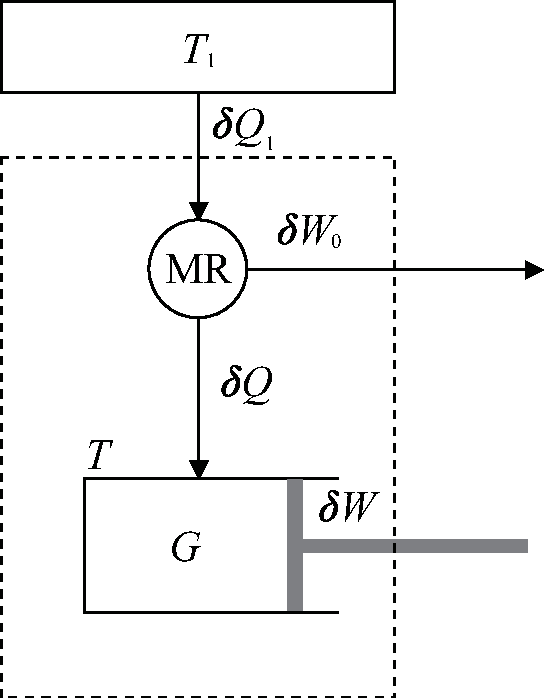
\includegraphics[width=0.5\linewidth]{pic/数学描述.pdf}
		\caption{数学描述装置图}
		\label{数学描述}
\end{minipage}
\begin{minipage}{0.5\linewidth}
		\centering
		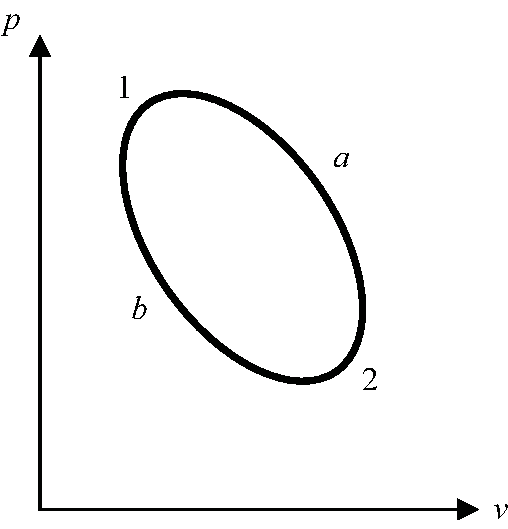
\includegraphics[width=0.62\linewidth]{pic/数学描述曲线.pdf}
		\caption{数学描述循环曲线图}
		\label{数学描述曲线}
\end{minipage}
\end{figure}
\vspace*{-1em}
\begin{itemize}
	\item 设计装置如图\ref{数学描述}.循环曲线如图\ref{数学描述曲线}.\vspace*{-0.5em}
\begin{itemize}
	\item 正循环$(1-a-2-b-1)$
	\begin{itemize}
		\item 热机从热源吸热$\delta Q_1$,向$G$放热$\delta Q$,对外输出循环功$\delta W_0 = \delta Q_1 - \delta Q$
		\item 系统$G$从热机吸热$\delta Q$,对外做功$\delta W$
		\item 整个系统对外输出的微量总功$\delta W_T = \delta W_0 + \delta W$,循环总功为
		\begin{align}
			W_T = \oint \delta W_0 + \oint \delta W
		\end{align}
	由循环的能量方程和静止闭系$G$的能量方程
	\begin{align}
		\begin{aligned}
			\delta W_0 &= \delta Q_1 - \delta Q \\
			\delta W &= \d Q - \d U_G 
		\end{aligned}
	\quad \Longrightarrow \quad
	W_T = \oint \left(\delta Q_1 - \delta Q\right) + \oint \left(\d Q - \d U_G \right) = \oint \left(\delta Q_1 - \d U_G\right) 
	\end{align}
由于$\displaystyle \oint \d U_G = 0$,所以
\begin{align}
	W_T = \oint \delta Q_1
\end{align}
这说明正循环的过程中,整个机器从单一热源吸热$\displaystyle \oint \delta Q_1$并使之完全变为功$W_T$,而没有引起其他变化。根据开氏说法,这是不可能实现的。
	\end{itemize}
	\item 逆循环$(2-b-1-a-2)$\\	
		\hspace*{2em} 开氏说法认为,如果这个系统进行逆循环,使外界对机器提供总功$W_T$,并使之全部转换为热$\oint \delta Q_1$转移到$T_1$中去是能实现的。因此,在这种机器中,只能有
		\begin{align}
			\oint \delta Q_1 \le 0
		\end{align}
\end{itemize}	
\end{itemize}

对于\dy[卡诺机]{KNJ}MR,其效率可以表示为
\begin{align}
	\eta = \dfrac{\delta W_0}{\delta Q_1} = \dfrac{\delta Q_1 - \delta Q}{\delta Q_1} = \dfrac{T_1 - T}{T_1}
\end{align}
由此可得
\begin{align}
	\delta Q_1 = T_1 \dfrac{\delta Q}{T}
\end{align}
即
\begin{align}
	\oint \dfrac{\delta Q}{T} \le 0
\end{align}
称为\dy[克劳修斯积分]{KLXS}。其中
\begin{myitemize}
	\item $\displaystyle \oint \dfrac{\delta Q}{T} = 0$ 代表可逆过程
	\item $\displaystyle \oint \dfrac{\delta Q}{T} < 0$ 代表不可逆过程
	\vspace*{0.3em}
\end{myitemize}


\section{熵}
\subsection{概念引入}
对于可逆过程,由克劳修斯积分可知$\displaystyle \oint \dfrac{\delta Q}{T} = 0$,那么$\dfrac{\delta Q}{T}$一定是系统中工质的状态量的分量。

\defination[熵]
在可逆状态下,令
\begin{align}
	\d S = \dfrac{\delta Q}{T}
\end{align}
新的状态参数$S$称为\dy[熵]{S},$\delta Q$为可逆过程中交换的微量热量,$T$为可逆过程中的系统温度。

\subsection{熵的特点}
\begin{itemize}
	\item 熵$S$为状态参数中的广延参数
	\item 单位质量工质的熵$s = \dfrac{S}{m}$称为\dy[比熵]{BS}
	\item 单位物质的量工质的熵$s = \dfrac{S}{n}$称为\dy[摩尔熵]{MES}
\end{itemize}
	\begin{figure}[!htb]
	\centering
	\begin{tikzpicture}
		\node(A) [draw, inner sep = 6pt]{熵是状态参数};
		\node(B) [draw, inner sep =6pt, below of = A , node distance = 1.25cm]{若状态确定,则熵确定};
		\node(C) [draw , inner sep =6pt, below of=B, node distance = 1.25cm]{若过程初态和终态确定,则熵变确定};
		\node(D) [draw , inner sep =6pt, below of=C, node distance = 1.25cm]{同一初态到同一终态的各种过程熵变相同};
		
		\draw[arrows={-Stealth[scale=0.8]}] (A) -- (B);
		\draw[arrows={-Stealth[scale=0.8]}] (B) -- (C);
		\draw[arrows={-Stealth[scale=0.8]}] (C) -- (D);
	\end{tikzpicture}
	\caption{熵与熵变的特点}
\end{figure}
\vspace*{-1.5em}

\section{熵变}
\begin{equation*}
	\mbox{熵变}\,\,
	\begin{cases}
		\,\,\mbox{可逆过程的熵变———通过熵变定义式来计算}\\
		\,\,\mbox{不可逆过程的熵变———通过构造相应的可逆过程来计算}
	\end{cases}
\end{equation*}
\vspace*{1em}
\subsection{理想气体的熵变}
由静止简单可压闭系理想气体的能量方程和理想气体状态方程,
\begin{align*}
\d s &= \dfrac{\delta q}{T}\\
\delta q &= C_V\,\d T + p \,\d v 
\quad \Longrightarrow \quad \d s = C_V \dfrac{\d T}{T} + R \dfrac{\d v}{v}
\quad \Longrightarrow \quad \Delta s = C_V \ln \dfrac{T_2}{T_1} + R \ln \dfrac{v_2}{v_1}
\quad \Longrightarrow \quad \Delta S = m \delta s \\
p &= \dfrac{RT}{v}
\end{align*}
同理,我们可以得到

\begin{table}[!htb]
	\centering\setlength{\tabcolsep}{12mm}{
		\begin{tabular}{cc}
			\toprule
			微分形式 & 积分形式\\
			\midrule
			& 	\vspace*{-1em}
			\\
			$\displaystyle \d s = C_v\dfrac{\d T}{T} + R \dfrac{\d v}{v}$ & $\displaystyle \Delta s = C_V \ln \dfrac{T_2}{T_1} + R \ln \dfrac{v_2}{v_1}$\\[1em]
			$\displaystyle \d s = C_p \dfrac{\d T}{T} - R \dfrac{\d p}{p}$ & $\displaystyle C_p \ln \dfrac{T_2}{T_1} - R \ln \dfrac{p_2}{p_1}$\\[1em]
			$\displaystyle \d s = C_p \dfrac{\d v}{v} + C_v \dfrac{\d p}{p}$ & $\displaystyle \Delta s =C_p \ln \dfrac{v_2}{v_1} + C_V\ln \dfrac{p_2}{p_1}$\\[1em]
			\bottomrule
		\end{tabular}
	\caption{理想气体可逆过程的比焓变计算公式}
	}
\end{table}

\begin{figure}[!htb]
	\noindent 对于特殊的热力过程,有
\end{figure}

\begin{table}[!htb]
	\centering\setlength{\tabcolsep}{8mm}{
		\begin{tabular}{cccc}
			\toprule
			过程 & 过程特点 & 比熵变微分式 & 比熵变积分式\\
			\midrule
			& 	&  &\vspace*{-1em}
			\\
			定温 & $\displaystyle \d T =0$ & $\d s = R \dfrac{\d v}{v} = -R \dfrac{\d p}{p}$ & $\displaystyle \Delta s = R \ln \dfrac{v_2}{v_1} = - R \dfrac{p_2}{p_1}$\\[1em]
			定容 & $\displaystyle \d v = 0$ &$\displaystyle \d s = C_V \dfrac{\d T}{T} = C_V \dfrac{\d p}{p}$ & $\displaystyle \Delta s = C_V \ln \dfrac{T_2}{T_1} = C_V \ln \dfrac{p_2}{p_1}$\\[1em]
			定压 &$\displaystyle \d p = 0$ &$\displaystyle \d s = C_p \dfrac{ \d T}{T} = C_p \dfrac{\d v}{v}$ & $\displaystyle \Delta s = C_p \ln \dfrac{T_2}{T_1} = C_p \ln \dfrac{v_2}{v_1}$\\[1em]
			绝热 & $\displaystyle \delta q = 0$ & $\displaystyle \d s = 0 $& $\displaystyle \Delta s =0$\\[0.5em]
			\bottomrule
		\end{tabular}
		\caption{理想气体特殊热力学过程的比焓变计算公式}
	}
\end{table}

\noindent \textbf{理想气体$T-s$图的斜率}
由理想气体的热量计算公式\eqref{理想气体热量计算},有
\begin{align*}
	\delta q = \dfrac{n - k}{n - 1}C_V\d T = T \d s
\end{align*}
故
\begin{align}
	\dfrac{\d T}{\d s} = \dfrac{n - k}{n - 1} \dfrac{C_V}{T}
\end{align}
\begin{enumerate}[(1) ]
	\item 定容过程:$n=\pm \infty, \dfrac{\d T}{\d s} = \dfrac{T}{C_V} $
	\item 定压过程:$n=0, \dfrac{\d T}{\d s} = \dfrac{T}{C_p} $
	\item 定温过程:$n=1, \dfrac{\d T}{\d s} = 0 $
	\item 绝热过程:$n=k, \dfrac{\d T}{\d s} \to \infty $
\end{enumerate}

\subsection{不可压缩物质的熵变}
对于不可压缩的物质,其比热容一般变化不大,通常设定为常数,则
\begin{align*}
	\begin{aligned}
		\d s &= \dfrac{\delta q}{T}\\
		\delta q &= C\,\d T 
	\end{aligned}
	\quad \Longrightarrow \quad \d s = C \dfrac{\d T}{T} 
	\quad \Longrightarrow \quad \Delta s = C \ln \dfrac{T_2}{T_1} 
	\quad \Longrightarrow \quad \Delta S = m C \ln \dfrac{T_2}{T_1} 
\end{align*}

\subsection{封闭系统的熵变}
假定系统经历的过程在可逆和不可逆两种情况下进行
\begin{align*}
	\begin{aligned}
		\d s &= \dfrac{\delta q_{\text{R}}}{T}\\
		\delta q_{\text{R}} &= \d u_{\text{R}} + \d w_{\text{R}}\\
		\delta q_{\text{I}} &= \d u_{\text{I}} + \d w_{\text{I}}\\
	\end{aligned}
	\quad \xrightarrow{\quad \textstyle \Delta = \delta w_{\text{R}}- \delta w_{\text{I}}\quad} \quad \d s =  \dfrac{\d q_{\text{I}}}{T} + \dfrac{\Delta }{T}
	\quad \xrightarrow[\quad \textstyle 、\d s_{\text{g}} = \dfrac{\Delta}{\d T} \quad]{\quad \textstyle \d s_{\text{f}} = \dfrac{\d q_{\text{I}}}{\d T} \quad }\quad \d s = \textstyle \d s_{\text{f}} + s_{\text{g}}	
\end{align*}
即
\begin{equation}
	\mbox{封闭系统的熵变} = \mbox{热量熵流} + \mbox{熵产}
\end{equation}
其中,$\Delta$称为\dy[功耗]{GH},它是由不可逆因素引起的功损失。

\subsection{开放系统的熵变}
\begin{align*}
	\mbox{开放系统的熵变}\,\,
	\begin{cases}
		\,\,\mbox{质量熵流}\\
		\,\,\mbox{热量熵流}\\
		\,\,\mbox{熵产}
	\end{cases}
\end{align*}
\noindent 所以
\begin{itemize}
	\item 对于单个入口和单个出口
	\begin{align}
		\d S_{\text{C.V.}}= \left(\delta s_1 m_1 - \delta s_2 m_2\right)  + \d S_{\text{f}}+ \d S_{\text{g}}
	\end{align}
	\item 对于多个入口和多个出口
	\begin{align}
		\d S_{\text{C.V.}}= \left( \sum_i \delta s_{1i} m_{1i} - \sum_j \delta s_{2j} m_{2j}\right)  + \d S_{\text{f}}+ \d S_{\text{g}}
	\end{align}
	\item 对于稳定流动系统,有
	\begin{align*}
		\d S_{\text{C.V.}} = 0\\
		\delta m_1 = \delta m_2 = \delta m
	\end{align*}
	所以
	\begin{align}
		0 = (s_1 - s_2)\delta m + \d S_{\text{f}}+ \d S_{\text{g}}\\
		\d S =  (s_2 - s_1)\delta m = \d S_{\text{f}}+ \d S_{\text{g}}
	\end{align}
	即\textbf{稳定流动开放系统的工质流过控制体的熵变$\,=\,$热量熵流$\,+\,$熵产}
\end{itemize}

\subsection{质量转换系统的熵变}
由熵的定义式及质量转换系统的热量计算公式,有
\begin{align}
	\begin{aligned}
		\d S &=\dfrac{\delta Q}{T}\\
		\delta Q &= \d U + \sum_j F_j\,\d X_j - \sum_i \mu_i \, \d m_i
	\end{aligned}
\quad \Longrightarrow \quad 
\d S = \dfrac{1}{T} \,\d U + \dfrac{1}{T} \sum_j F_j\,\d X_j - \dfrac{1}{T} \sum_i \mu_i \, \d m_i
\end{align}

\subsection{等温过程的熵变}
\noindent 1. \dy[热源]{RY}和\dy[冷源]{LY}是特殊的热力系统
\begin{itemize}
	\item \dy[恒温热源]{HWRY} \quad 在与工质交换热量时温度保持不变的热源
	\item \dy[恒温冷源]{HWLY}\quad 在与工质交换热量时温度保持不变的冷源
	\item 举例\quad \textbf{大气环境可看作恒温热源或恒温冷源}
	\begin{align}
		\Delta S = \int \dfrac{\delta Q}{T} = \dfrac{1}{T} \int \delta Q = \dfrac{Q}{T}
	\end{align}
\end{itemize}

\noindent 2. \dy[相变过程]{XBGC}中物质状态变化是在等温条件下进行的
\begin{itemize}
	\item 相变过程中的热效应统称为相变潜热,以$\gamma$表示,单位为J/kg.
	\item 举例 \quad \textbf{气化热、熔解热}
	\begin{align}
		\Delta S = \int \dfrac{\delta Q}{T} = \dfrac{1}{T} \int \delta Q = \dfrac{m \gamma}{T}
	\end{align}
\end{itemize}

\subsection{不可逆过程的熵变}
\section{熵增原理}

\subsection{熵增原理}
\noindent 我们已经知道

\begin{itemize}
	\item 封闭系统的熵变 \quad $\d S = \d S_{\text{f}} + \d S_\text{g}$
	\item 开放系统的控制体的熵变 \quad $\displaystyle \d S_{\text{C.V.}} = \sum_i s_{1i}\delta m_{1i} - \sum_j s_{2j} \delta m_{2j} + \d S_{\text{f}} + \d S_{\text{g}}$
\end{itemize}

\ttheorem[熵增原理]
对于孤立系统,孤立系统的熵变只用熵产,没有质量熵流和热量熵流,即
\begin{align}
	\d S = \d S_{\text{g}}
\end{align}
由$\d S_{\text{g}} \ge 0 \Rightarrow \d S \ge 0$,即可以表述为:\textbf{孤立系统的熵只能增加或不变,而不能减少},这个结论称为\dy[熵增原理]{SZYL}。

\warn[
熵增原理的适用性
\begin{itemize}
	\item 熵增原理\textcolor{red}{适用于孤立系统}
	\item 熵增原理还\textcolor{red}{适用于绝热封闭系统}
	\item 熵增原理\textcolor{red}{不一定适用于一般的封闭系统}
	\item 熵增原理\textcolor{red}{不一定适用于一般的开放系统}
\end{itemize}
]

\subsection{熵增原理的应用}
\vspace*{-1em}

\example[判断循环可行与否]
欲设计一热机,使之能从温度为973K的高温热源吸热2000KJ,并向温度为303K的低温冷源放热800KJ,问此循环可行与否?

\solve
方法一:利用熵增原理
\begin{align*}
	\Delta S = \Delta S_{\text{H}} + \Delta S_{\text{L}} + \Delta S_{\text{sys}} + \Delta S_{\text{sur}} = \dfrac{-2000}{973} + \dfrac{800}{303} + 0 + 0 = 0.585\,\text{kJ/K} > 0
\end{align*}
其中,
\begin{myitemize}
	\item $\Delta S$ \quad 系统的总熵变
	\item $\Delta S_{\text{H}}$ \quad 高温热源$T_1$的熵变
	\item $\Delta S_{\text{L}}$ \quad 低温热源$T_2$的熵变
	\item $\Delta S_{\text{sys}}$\quad 工质在循环过程中的熵变
	\item $\Delta S_{\text{sur}}$\quad 环境的熵变\vspace*{0.3em}
\end{myitemize}

\solveother 
方法二:克劳修斯积分
\begin{align*}
	\oint \dfrac{\delta Q}{T} = \int \dfrac{\delta Q_1}{T_1} + \int \dfrac{\delta Q_2}{T_2} = \dfrac{2000}{973} - \dfrac{800}{303} = -0.585\,\text{kJ/K} > 0
\end{align*}

\example[判断过程是否可逆]
欲设计一热机,使之能从温度为973K的高温热源吸热2000KJ,并向温度为303K的低温冷源放热800KJ,问此循环可逆与否?

\solve
方法一:利用熵增原理
\begin{align*}
	\Delta S_{\text{H}} + \Delta S_{\text{L}} + \Delta S_{\text{sys}} + \Delta S_{\text{sur}} = \dfrac{-2000}{973} + \dfrac{800}{303} + 0 + 0 = 0.585\,\text{kJ/K} \neq 0
\end{align*}

\solveother 
方法二:克劳修斯积分
\begin{align*}
	\oint \dfrac{\delta Q}{T} = \int \dfrac{\delta Q_1}{T_1} + \int \dfrac{\delta Q_2}{T_2} = \dfrac{2000}{973} - \dfrac{800}{303} = -0.585\,\text{kJ/K} \neq 0
\end{align*}
所以,该循环不可逆。

总结:判断循环是否可逆,只需要判断熵增$\d S$是否为0即可。
\vspace*{1.5em}

\example[热动力系统]
任何热动力装置,都可以用图表示,取孤立系统后,其熵变为
\begin{align*}
	\Delta S &= \Delta S_1 + \Delta S_2 + S_{\text{sys}} \\
	& = -\dfrac{Q_1}{T_1} + \dfrac{Q_2}{T_2}\\
	& = \dfrac{Q_2}{T_2} - \dfrac{Q_1}{T_1}
\end{align*}
根据循环过程的能量方程,$Q_2 = Q_1 - W_0$,所以
\begin{align}
	\Delta S = Q_1 \left(\dfrac{1}{T_2} - \dfrac{1}{T_1} - \dfrac{W_0}{T_2}\right)
\end{align}
令$\Delta S = 0$,则求出最大功量为
\begin{align}
	W_{0, \max} = Q_1\left(\dfrac{1}{T_2} - \dfrac{1}{T_1}\right)T_2 = Q_1\left(1 - \dfrac{T_2}{T_1}\right)
\end{align}
若已知所需的功量为$W_0$,在可逆条件下,可以求得最小热量
\begin{align}
	Q_{1, \min} = W_0 \left(\dfrac{T_1}{T_1 -T_2}\right)
\end{align}
根据最小热量可以确定最低限度的燃料需要量。
	\begin{figure}[!htb]
		\centering 
		\begin{minipage}{0.4\linewidth}
			\centering
			\begin{tikzpicture}
				\node(A) [draw, inner sep = 6pt]{$\quad\quad T_1 \quad \quad $};
				\node[circle] (B) [draw, inner sep = 8pt, below of = A, node distance = 1.5cm]{};
				\node(C) [draw, inner sep =6pt, below of = A , node distance = 3cm]{$\quad \quad T_2 \quad \quad $};
				
				\draw[arrows={-Stealth[scale=0.8]}] (A) -- (B)node[midway,xshift = -3mm]{$Q_1$};
				\draw[arrows={-Stealth[scale=0.8]}] (B) -- (C) node[midway,xshift = -3mm]{$Q_2$};
				\draw[arrows={-Stealth[scale=0.8]}] (B) -- +(1.5cm, 0cm)node[near end, above = 0cm]{$W_0$};
			\end{tikzpicture}
			\caption{制热系统装置图}
			\label{制热系统}
		\end{minipage}
		\begin{minipage}{0.4\linewidth}
			\centering
			\begin{tikzpicture}
				\node(A) [draw, inner sep = 6pt]{$\quad\quad T_1 \quad \quad $};
				\node[circle] (B) [draw, inner sep = 8pt, below of = A, node distance = 1.5cm]{};
				\node(C) [draw, inner sep =6pt, below of = A , node distance = 3cm]{$\quad \quad T_2 \quad \quad $};
				
				\draw[arrows={-Stealth[scale=0.8]}] (A) -- (B)node[midway,xshift = 3mm]{$Q_1$};
				\draw[arrows={-Stealth[scale=0.8]}] (B) -- (C) node[midway,xshift = 3mm]{$Q_2$};
				\draw[arrows={-Stealth[scale=0.8]}] (-1.5cm, -1.5cm) -- +(B)node[near start, above =0cm]{$W_0$};
			\end{tikzpicture}
			\caption{制冷系统装置图}
			\label{制冷系统}
		\end{minipage}
	\end{figure}
\vspace*{1em}

\example[制冷系统]
制冷装置如图\ref{制冷系统}所示,构成孤立系后,由熵的定义和能量方程可得
\begin{align*}
		\Delta S = \dfrac{Q_1}{T_1} - \dfrac{Q_2}{T_2}\\[0.5em]
		Q_1 = W_0 + Q_2
\end{align*}
即
\begin{align*}
	\Delta S & = \dfrac{W_0 + Q_2}{T_1} - \dfrac{Q_1}{T_2}\\[0.5em]
	& = \dfrac{W_0}{T_1} + Q_2\left(\dfrac{1}{T_1} - \dfrac{1}{T_2} \right)
\end{align*}
若已知所需的制冷量$Q_2$,令$\Delta S = 0$,可以得到最小功量为
\begin{align}
	W_{0, \min} = Q_2 \left(\dfrac{T_1}{T_2} - 1\right)
\end{align}
若已知所能提供的功量为$W_0$,令$\Delta S = 0$,可以得到最多制冷量为
\begin{align}
	Q_{2, \max} = W_0\left(\dfrac{T_2}{T_1 - T_2} \right)
\end{align}
\vspace*{1em}

\subsection{熵增原理的本质}
\textbf{熵增原理是热力学第二定律的统一的数学描述,一切陈述方式都可包含在熵增原理之中。}
\begin{enumerate}
	\item 克氏说法与熵增原理\\
	熵增原理可推出克氏说法
	\begin{itemize}
		\item 设计装置如图\ref{克氏熵增}.
		\item 证明:在熵增原理的条件下若假设克氏说法不成立,即低温物体A自动向高温物体B传热$\delta Q$,则有
		\begin{align*}
			\d S = \d S_\text{A} + \d S_\text{B} = - \dfrac{\delta Q}{T_\text{A}} + \dfrac{\delta Q}{T_\text{B}} = \delta Q \left(\dfrac{1}{T_{\text{b}}} - \dfrac{1}{T_\text{A}}\right)<0
		\end{align*}
	这与熵增原理矛盾,故假设不成立,故克氏说法成立。
	\end{itemize}	

\begin{figure}[!htb]
	\centering 
	\begin{minipage}{0.45\linewidth}
		\centering
		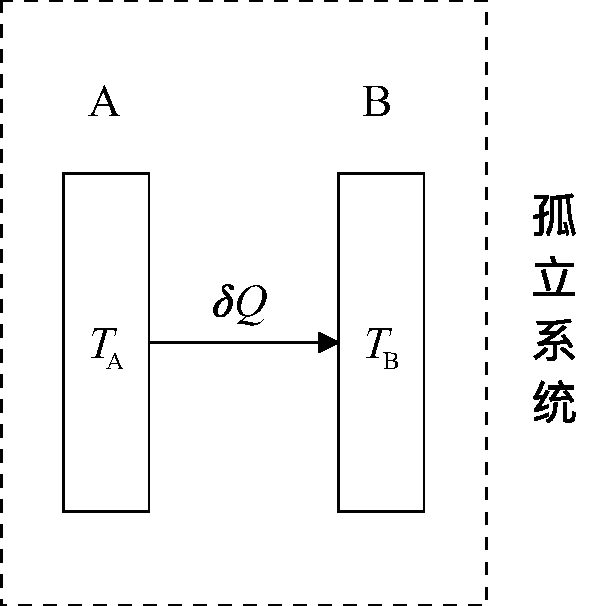
\includegraphics[width=0.6\linewidth]{pic/熵增本质克.pdf}
		\caption{克氏熵增图}
		\label{克氏熵增}
	\end{minipage}
	\begin{minipage}{0.45\linewidth}
		\centering
		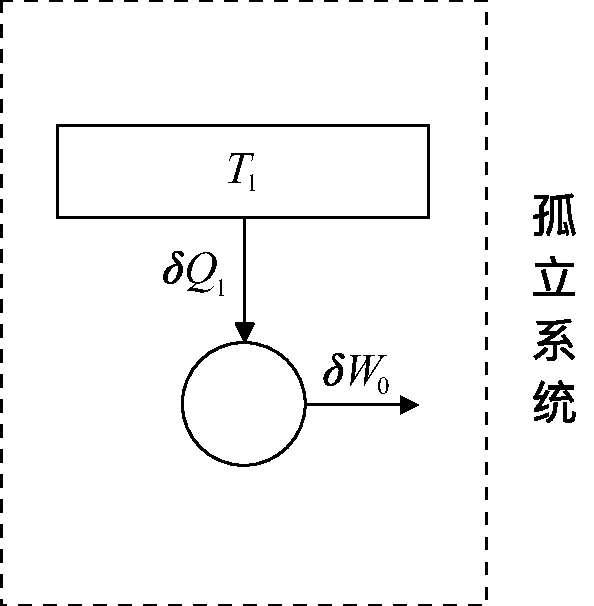
\includegraphics[width=0.6\linewidth]{pic/熵增本质开.pdf}
		\caption{开氏熵增图}
		\label{开式熵增}
	\end{minipage}
\end{figure}

	\item 开氏说法与熵增原理\\
	熵增原理可推出开氏说法
	\begin{itemize}
		\item 设计装置如图\ref{开式熵增}.
		\item 证明:在熵增原理的条件下若假设开氏说法不成立,即工质在循环过程中从单一热源吸热且完全转换为功而不引起其他变化,则有
		\begin{equation*}
			\d S = \d S_{\text{T}_1} + \d S_{\text{sys}} + \d S_{\text{sur}} = - \dfrac{\delta Q_1}{T_\text{A}} + \dfrac{\delta Q}{T_\text{B}} = \dfrac{\delta Q_1}{T_{\text{1}}} + 0 + 0= -\dfrac{\delta Q_1}{T_1}<0
		\end{equation*}
		这与熵增原理矛盾,故假设不成立,故开氏说法成立。
	\end{itemize}	
\end{enumerate}

\subsection{熵增原理的推论}
\begin{enumerate}
	\item 孤立系统或绝热封闭系统中,质量守恒、能量守恒,但熵不守恒,且只增不减。
	\item 若所假设过程使孤立系统或绝热封闭系统熵减少,则它不能自动进行,除非使过程逆向进行或补偿另外的熵增加的过程。
	\item 孤立系统处于平衡状态时,熵具有最大值。因为孤立系统中任何非平衡状态必将引发不可逆过程并自动趋向平衡状态,该不可逆过程进行时熵不断增加,到达平衡状态时熵值达到最大并保持不变。
	\begin{align}
		\d S \equiv 0\quad \quad \quad \quad \mbox{(平衡的熵判据)}
	\end{align}
\end{enumerate}

\section{能量可用性}
\subsection{能量可用性的概念}
\begin{table}[!htb]
	\centering\setlength{\tabcolsep}{10mm}{
		\begin{tabular}{ccc}
			\toprule
			转换不受限制的能量 & 转换受到一定限制的能量 & 不可转换的能量\\
			\midrule
			\makecell[c]{电能,宏观动能\\宏观势能,轴功
}& 热量,热力学能,焓
 & \makecell[c]{环境介质的\\热力学能}\\
			\hline
			可用能 (㶲) & 可用能(㶲)$+$不可用能(㷻)& 不可用能(㷻)\\
			\bottomrule
		\end{tabular}
		\caption{能量可用性的分类}
	}
\end{table}

\textbf{一切能量形式由\dy[㶲]{Y}(可用能)和\dy[㷻]{W}(不可用能)组成,㶲是能量可用性的度量。}
\vspace*{0.5em}

\subsection{可逆条件下的能量可用性}

\noindent \textbf{1. 可逆条件下热量的㶲和㷻}
	\begin{figure}[!htb]
		\centering
		\begin{minipage}{0.45\linewidth}
			\centering
			\begin{tikzpicture}
				\node(A) [draw, inner sep = 6pt]{$\quad\quad T_1 \quad \quad $};
				\node[circle] (B) [draw, inner sep = 8pt, below of = A, node distance = 1.5cm]{};
				\node(C) [draw, inner sep =6pt, below of = A , node distance = 3cm]{$\quad \quad T_2 \quad \quad $};
				
				\draw[arrows={-Stealth[scale=0.8]}] (A) -- (B)node[midway,xshift = -3mm]{$Q_1$};
				\draw[arrows={-Stealth[scale=0.8]}] (B) -- (C) node[midway,xshift = -3mm]{$Q_2$};
				\draw[arrows={-Stealth[scale=0.8]}] (B) -- +(1.5cm, 0cm)node[near end, above = 0cm]{$W_0$};
			\end{tikzpicture}
			\caption{热机装置图}
			\label{热机}
		\end{minipage}
		\begin{minipage}{0.45\linewidth}
			\centering
			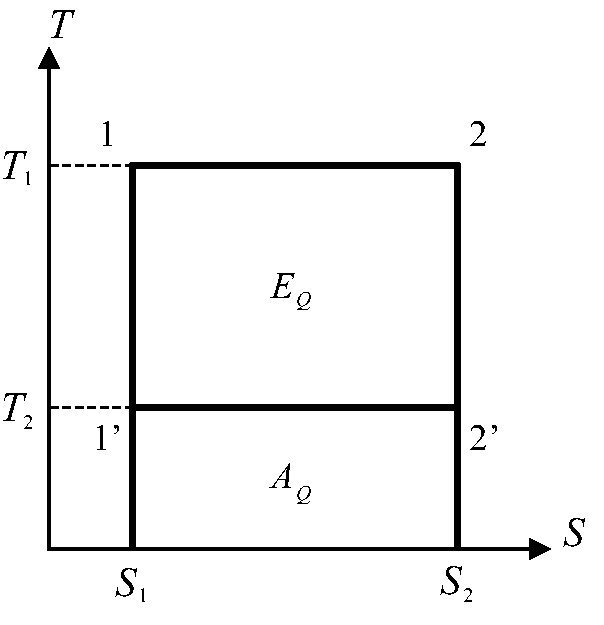
\includegraphics[width=0.6\linewidth]{pic/㶲㷻TS图.pdf}
			\vspace*{-1.5em}
			\caption{㶲㷻在$T-S$图上的表示}
			\label{㶲㷻TS图}
		\end{minipage}
	\end{figure}

\noindent 对于由热转换为功的热机(如图\ref{热机}.),热源为$T_1$,冷源为$T_2$,
\begin{itemize}
	\item 在可逆条件下,输出的最大功量为$W_{0, \max} = Q_1 \left(1 - \dfrac{T_2}{T_1}\right)$
	\item 当冷源温度达到$T_0$(最低温度限)时,$Q_1$中最大的可转换值为$Q_1 \left(1 - \dfrac{T_0}{T_1}\right)$,即$Q_1$的㶲为$E_{Q_1} = Q_1 \left(1 - \dfrac{T_0}{T_1}\right)$
	\item $Q_2$的㶲为$E_{Q_2} = Q_2 \left(1 - \dfrac{T_0}{T_2}\right)$
\end{itemize}
热量的㶲简称\dy[热㶲]{RY},用$E_Q$表示,温度$T$下释放热量$Q$的㶲为
\begin{align}
	E_Q = Q \left(1 - \dfrac{T_0}{T} \right)
\end{align}
所以,
\begin{align}
	Q = E_Q  + T_0 \dfrac{Q}{T}
\end{align}
热量的㷻简称\dy[热㷻]{RW},用$A_Q$表示,温度$T$下释放热量$Q$的㷻为
\begin{align}
	A_Q = T_0 \dfrac{Q}{T}
\end{align}
	由于$T$为恒温系统的温度,故有$\Delta S = \dfrac{Q}{T}$,则
	\begin{align}
		A_Q = T_0 \Delta S
	\end{align}
综上可得
\begin{itemize}
	\item 热量为热㶲与热㷻两部分之和,它们可以在$T-S$图上几何地表示出来,如图\ref{㶲㷻TS图}.
\begin{align}
	Q = E_Q + A_Q = Q \left(1 - \dfrac{T_0}{T} \right) + T_0 \Delta S
\end{align}
	\item 输出的循环功
	\begin{align}
		W_ 0 &= Q_1 - Q_2\notag \\
		& = \left(E_{Q_1} + A_{Q_1}\right) - \left(E_{Q_2} + A_{Q_2}\right) \notag \\
		& = E_{Q_1} - E_{Q_2} + T_0 \left(\dfrac{Q_1}{T_1} - \dfrac{Q_2}{T_2}\right)
	\end{align}
	对于可逆机,有
	\begin{align*}
		\dfrac{Q_1}{T_1} = \dfrac{Q_2}{T_2}
	\end{align*}
	所以
	\begin{align}
		W_0 = E_{Q_1} - E_{Q_2}
		\label{热㶲平衡方程}
	\end{align}
	式\eqref{热㶲平衡方程}称为\dy[热㶲平衡方程]{RYPHFC},说明可逆热机对外界所作的循环功等于工质吸收热量与放出热量中的热㶲的落差。
\end{itemize}

\noindent \textbf{2. 可逆条件下热力学能的㶲和㷻}
\begin{figure}[!htb]
	\centering
	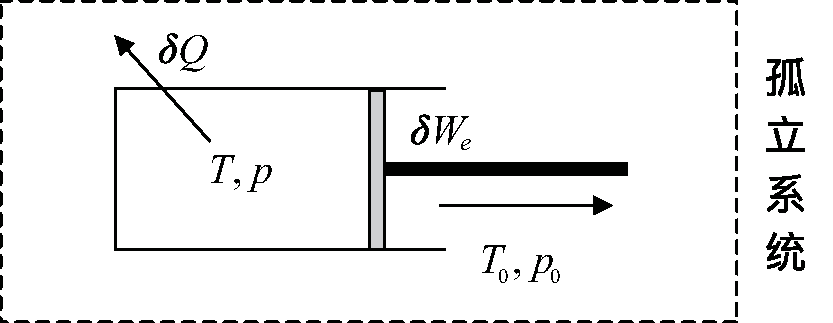
\includegraphics[width=0.4\linewidth]{pic/静止封闭系统.pdf}
	\caption{静止封闭系统}
	\label{静止封闭系统}
\end{figure}

\noindent 分析静止封闭系统如图\ref{静止封闭系统}.其中$T_0 < T, p_0 < p$.
\begin{itemize}
	\item 由热力学第一定律,得能量方程
	\begin{align*}
		- \delta Q = \d U + \delta W = \d U + p_0 \d V + \delta W_{\text{e}}
	\end{align*}
	\item 由可逆过程孤立系的熵变
	\begin{align*}
		\d S_{\scriptsize \text{孤}}  =  \d S + \d S_{\text{sur}} = 0 \quad \Rightarrow \quad  \d S = - \d S_{\text{sur}} = - \dfrac{- \delta Q}{T_0} \quad \Rightarrow \quad - \delta Q = T_0 \d S
	\end{align*}
	\item 联立两个方程,可以得到
	\begin{align}
		T_0 \d S = \d U + p_0 \d V + \delta W_{\text{e}}
	\end{align}
	积分,得
	\begin{align}
		T_0(S_0 - S) = U_0 - U + p_0(V_0 - V) + \int_{(T,p)}^{(T_0, p_0)} \delta W_{\text{e}}
	\end{align}
\end{itemize}
令$\displaystyle E_U = \int_{(T,p)}^{(T_0, p_0)} \delta W_{\text{e}} = W_{\text{e}}$,代表热力学能中可用部分,称为\dy[热力学能㶲]{RLXNY}。则
\begin{align}
	E_U = U - \left[U_0 + p_0 (V_0 - V) - T_0(S_0 - S)\right]
\end{align}
所以,内能也可以写为
\begin{align}
	U = E_U + \left[U_0 + p_0 (V_0 - V) - T_0(S_0 - S)\right]
\end{align}
其中,
\begin{myitemize}
	\item $U_0$为到达外界状态时系统剩余的热力学能
\vspace*{-0.7em}
	\item $p_0(V_0 - V)$为克服外界压力消耗的功量
\vspace*{-0.7em}
	\item $T_0(S - S_0)$为向外界放出的热量\vspace*{0.3em}
\end{myitemize}

\noindent 它们皆为不可用能量。
\newpage

令$A_U = U_0 + p_0 (V_0 - V) + T_0(S - S_0)$,它代表热力学能中不可用部分,称为\dy[热力学能㷻]{RLXNW}。

所以热力学能为热力学能㶲与热力学能㷻两部分之和,即
\begin{align}
	U = E_U + A_U
\end{align}
其中,
\begin{myitemize}
	\item 热力学能㶲$E_U = U - \left[U_0 + p_0 (V_0 - V) - T_0(S_0 - S)\right]$\vspace*{-0.7em}
	\item 热力学能㷻$A_U = U_0 + p_0 (V_0 - V) - T_0(S_0 - S)$\vspace*{0.3em}
\end{myitemize}

\noindent 对于过程$(T_1, p_1) \to (T_2, p_2)$,有
\begin{align*}
	& T_0 \d S  = \d U + p_0 \d V + \delta W_{\text{e}}\\
	\Rightarrow \,\,& T_0(S_2 - S_1) = (U_2 - U_1) + p_0 (V_2 - V_1) + W_{\text{e,1-2}} \\
	\Rightarrow \,\,& W_{\text{e,1-2}} = (U_1 - U_2) + p_0 (V_1 - V_2) - T_0(S_1 - S_2) \\
	\Rightarrow \,\,& W_{\text{e,1-2}} = \big\lbrace U_1 - [U_ 0 + p_0(V_0 - V_1) - T_0(S_0 - S_1)] \big \rbrace - \big\lbrace U_2 - [U_ 0 + p_0(V_0 - V_2) - T_0(S_0 - S_2)]  \big \rbrace\\
\end{align*}
所以
\begin{align}
	W_{\text{e,1-2}} = E_{U_1} - E_{U_2}
	\label{热力学能㶲平衡方程}
\end{align}
式\eqref{热力学能㶲平衡方程}称为\dy[热力学能㶲平衡方程]{RLXNYPHFC}。即静止封闭系统从初态到终态的可逆过程中对外界所作的有效功等于初态与终态的热力学能㶲的落差。

\section{热力学第二定律评述}












